\section{Background Information \& Research}

\subsection{What is Fuzzy Logic?}
Fuzzy logic is a ``natural'' way of expressing uncertain or qualitative information \cite{albertos1998fuzzy}. It is a form of logic that deals with approximate reasoning, as opposed to fixed, exact values, like those found in classical logic (where we may only have properties being true, or false). Instead of these strict truth values, fuzzy logic systems have a range of truth, between 0 and 1. This makes fuzzy logic much better for handling and sorting data, and is an excellent choice for many control system applications, due to the way it mimics human control logic. Lotfi Zadeh, who formalised fuzzy logic in 1965, states that the key advantages of fuzzy logic are that it allows us to make rational decisions in environments of imprecision, uncertainty, and partiality of truth, and to perform a wide variety of physical and mental tasks, without any measurements or computations \cite{zadeh1999computing}.\\[2mm]
\noindent 
In a classical set, the membership, $\mu_A(x)$ of $x$, of a set, $A$, in universe, $X$, is defined:

\begin{center}
\vspace{-3mm}
$ 
\mu_A(x) = \left\lbrace
\begin{array}{ll}
1, & $iff x $\in$ A$      \\
0, & $iff x $\notin$ A$   \\
\end{array} \right\rbrace $ 
\end{center}
\vspace{-2mm}
\noindent 
That is, the element is either in the set, or not. In a fuzzy set, however, we have grades of membership, which are real numbers in the interval, $\mu_A(x) \in [0,1]$. Every member of a set has a membership grade to that set, depicting how true the property represented by that set is, for the given member \cite{zadeh1965fuzzy}. The traditional syntax for representing members of a fuzzy set is given below (although a full working knowledge of fuzzy logic theory is not necessary for this project).
\vspace{-2mm}
\begin{center}
$A = \mu_A(x_1)/x_1 + ... + \mu_A(x_n)/x_n$
\end{center}
\vspace{-2mm}
The easiest way to observe the merits of fuzzy logic are to look at terms that we humans use in our everyday life, and attempt to map these are crisp functions. For instances, terms like ``hot'', ``cold'', ``tall'', ``short'', are all terms that we understand very well, and use often. However, if we were asked to give \textit{exact} values for tallness, or shortness, we would not be able to. At what cut-off point would a person change from being considered short, to being considered tall? Fuzzy logic helps to alleviate these impossible choices, by having varying differing degrees of membership, to certain properties. The example in figure \ref{fig:fuzExample} shows this using three linguistic variables to describe the height of a person. Instead of at one point being either tall, short, or medium height, we, at all times, belong to all properties, to a differing degree. 

\begin{figure}[ht!]
\begin{center}
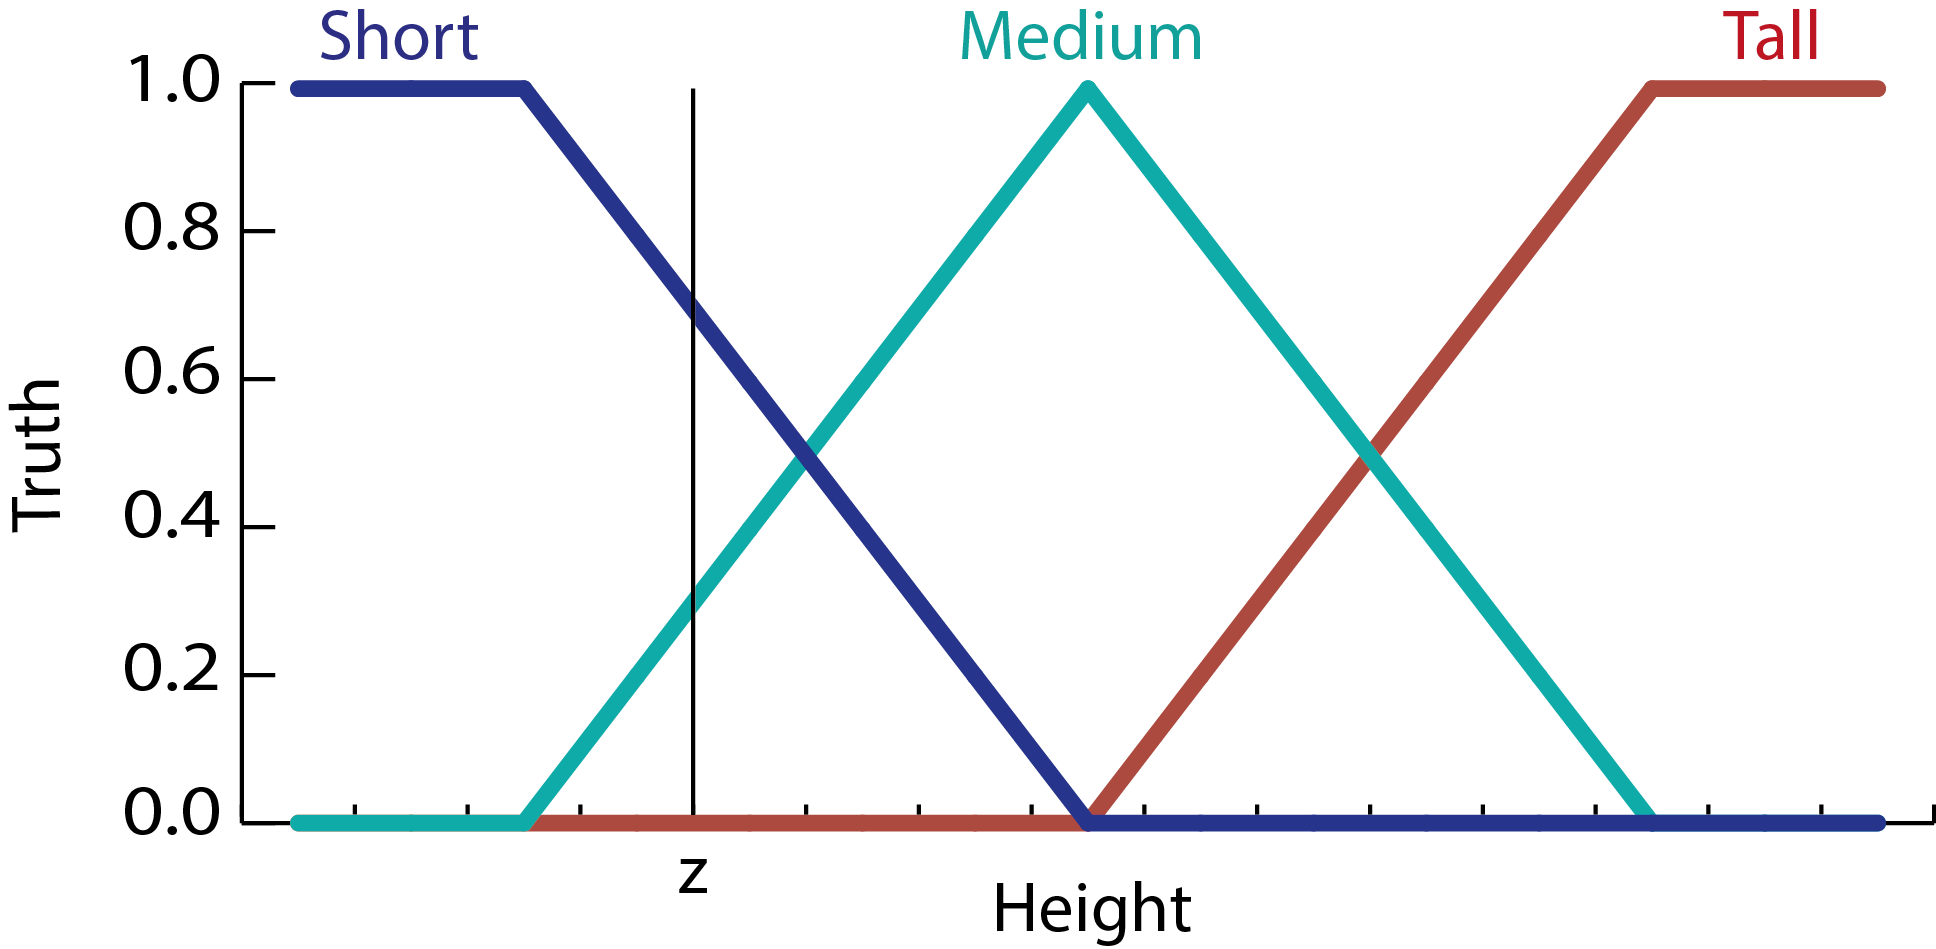
\includegraphics[width=0.6\textwidth]{images/fuzExample.png}
\end{center}
\vspace{-5mm}
\caption{A fuzzy set depicting ``height''}
\label{fig:fuzExample}
\end{figure}
\noindent
For instance, at the point labelled $z$, in the sets in figure \ref{fig:fuzExample}, we belong in the ``Short'' set, to degree 0.7, we belong in the ``Medium'' set, to degree 0.3, and we belong in the ``Tall'' set, to degree 0.0. This is, naturally, much more precise than simply saying we are ``Short'', ``Medium'', or ``Tall''.

\subsection{Existing Systems}
\label{sec:existing-systems}

{\color{red}\begin{enumerate}
\item Existing systems\\
{\color{red} Related work explaining what your project does that is new or is better than existing work in the same field}
	\begin{enumerate}
		\item FuzzyToolkitUoN
		\item MATLAB
		\item otheres... (see pres)
	\end{enumerate}
\end{enumerate}
}

\subsection{Platforms and Tools}
{\color{red}\begin{enumerate}
\item Languages used (R, Javascript)
\item Web technologies (tools, languages)
\item Shiny r to html
\item Bootstrap
\item jquery
\item Good user interfaces
\end{enumerate}}

